\documentclass[14pt,margin=0.72in,innermargin=-4.5in,blockverticalspace=-0.72in]{tikzposter}
\geometry{paperwidth=42in,paperheight=28.5in}
\usepackage[utf8]{inputenc}
\usepackage[T1]{fontenc}
\usepackage{amsmath}
\usepackage{amssymb}
\usepackage{graphicx}
\usepackage{adjustbox}
\usepackage{booktabs}
\usepackage{array}
\usepackage{enumitem}
\usepackage{uwtheme}
\usetikzlibrary{arrows.meta,positioning,calc}

\tikzposterlatexaffectionproofoff
\usetheme{UWTheme}
\usecolorstyle{UWStyle}

\usepackage[scaled]{helvet}
\renewcommand\familydefault{\sfdefault}
\definecolor{RandomBlue}{HTML}{2E86AB}
\definecolor{TargetOrange}{HTML}{F18F01}
\definecolor{KLPurple}{HTML}{7B2CBF}
\setlist[itemize]{leftmargin=1.0em,itemsep=0.02em,topsep=0.02em}
\setlength{\tabcolsep}{4pt}
\renewcommand{\arraystretch}{1.12}
\hyphenpenalty=10000
\exhyphenpenalty=10000
\sloppy
\raggedright

\title{Behavior Poisoning in Cooperative MAPPO}
\author{CS 763 Final Project Team}
\institute{University of Wisconsin--Madison}
\titlegraphic{
\includegraphics[width=0.10\textwidth]{uwlogocenter.png}}

\makeatletter
\renewcommand\TP@maketitle{%
   \centering
   \begin{minipage}[b]{0.8\linewidth}
        \centering
        \color{titlefgcolor}
        {\bfseries \huge \@title \par}
        \vspace*{0.25em}
        {\LARGE \@author \par}
        \vspace*{0.12em}
        {\Large \@institute}
    \end{minipage}%
    \tikz[remember picture,overlay]\node[anchor=south east,xshift=0.5\linewidth,inner sep=0pt] {%
       \@titlegraphic
    };
}
\makeatother

\newcommand{\tightcaption}[1]{\vspace{-0.42em}{\footnotesize\textbf{Caption.} #1}}
\newcommand{\minihead}[1]{\vspace{0.08em}\textbf{#1}}

\begin{document}
\maketitle
\centering

\block{Key finding: Behavior poisoning was not reliably harmful; effects were seed-sensitive, mixed, and non-monotonic in $p$.}{\vspace{-1.55em}}

\begin{columns}
    \column{0.31}
    \makeatletter\TP@blockverticalspace=4mm\makeatother

    \block{1. Motivation and Research Question}{
        In cooperative MARL, training data is not independent: each agent's learning signal depends on
        trajectories produced jointly with teammates. A compromised teammate can alter the training
        distribution for the whole team without touching rewards, observations, gradients, or weights.
        This is subtle because the attack disappears at evaluation; any effect must be learned from
        poisoned training rollouts.

        \innerblock{Research question}{
            Can action-level behavior poisoning during MAPPO rollout collection degrade final
            clean-evaluation performance in \texttt{simple\_spread}?
        }

        \textbf{Task.} In \texttt{simple\_spread}, three agents cover three landmarks while avoiding
        unnecessary collisions. Good coordination spreads agents across distinct landmarks.

        \begin{center}
\resizebox{0.72\linewidth}{!}{
        \begin{tikzpicture}[
            x=1cm, y=1cm,
            agent/.style={circle, draw=RandomBlue!85!black, fill=RandomBlue!18, very thick,
                          minimum size=0.62cm, inner sep=0pt, font=\bfseries\small},
            landmark/.style={circle, draw=GreyDark, fill=GreyBlue!30, thick,
                             minimum size=0.58cm, inner sep=0pt},
            cleanarrow/.style={-{Latex[length=2.7mm]}, very thick, RandomBlue!85!black},
            poisonarrow/.style={-{Latex[length=2.7mm]}, very thick, dashed, TargetOrange!95!black},
            callout/.style={font=\scriptsize, align=center, text=black},
            orangecallout/.style={font=\scriptsize, align=center, text=TargetOrange!95!black}
        ]
            \node[font=\scriptsize\bfseries, text=GreyDark] at (3.4,4.42)
                {Goal: spread agents across landmarks};
            \draw[rounded corners=6pt, line width=1.0pt, GreyDark, fill=white] (0,0) rectangle (6.8,4.15);

            \node[landmark] (L0) at (1.15,3.20) {};
            \node[font=\small] at (1.15,3.74) {L0};
            \node[landmark] (L1) at (5.65,3.20) {};
            \node[font=\small] at (5.65,3.74) {L1};
            \node[landmark] (L2) at (4.15,1.05) {};
            \node[font=\small] at (4.15,0.48) {L2};

            \node[agent] (A0) at (1.25,1.05) {A0};
            \node[agent] (A1) at (5.45,1.05) {A1};
            \node[agent] (A2) at (3.35,3.25) {A2};
            \draw[TargetOrange!95!black, very thick] (A0) circle (0.48);

            \draw[cleanarrow] (A2.west) -- ++(-0.82,-0.05) -- (L0.east);
            \draw[cleanarrow] (A1.north) -- (L1.south);
            \draw[cleanarrow] (A0.east) -- (L2.west);
            \draw[poisonarrow] (A0.north east) -- ++(0.85,0.95);

            \node[orangecallout] at (2.55,2.36)
                {training-time\\action replacement};
    \node[orangecallout, anchor=west] at (0.05,-0.38)
        {A0 training action may be replaced};
    \node[callout, anchor=east] at (6.75,-0.38)
        {Eval: gate OFF};
        \end{tikzpicture}}
        \end{center}

        {\small\textbf{Core idea.} Training-time action replacement $\rightarrow$ changed rollout
        distribution $\rightarrow$ seed-dependent clean-evaluation outcome.}
        \vspace{0.2em}

    }

    \block{2. Threat Model and Attack Mechanics}{
        \begin{center}
        \resizebox{0.39\linewidth}{!}{
        \begin{tikzpicture}[
            node distance=0.42cm,
            box/.style={draw=GreyDark, rounded corners=3pt, line width=0.8pt, align=center,
                        fill=GreyBlue, minimum height=0.7cm, text width=3.0cm, font=\small},
            attack/.style={draw=UWRed, rounded corners=3pt, line width=1pt, align=center,
                           fill=LightYellow, minimum height=0.7cm, text width=3.0cm, font=\small},
            eval/.style={draw=KellyGreen, rounded corners=3pt, line width=1pt, align=center,
                         fill=white, minimum height=0.7cm, text width=3.0cm, font=\small},
            arrow/.style={-{Latex[length=2.5mm]}, line width=0.9pt}
        ]
            \node[box] (a) {clean policy samples\\$a_{0,t}$};
            \node[attack, right=of a] (z) {poison gate\\$z_t\sim Bernoulli(p)$};
            \node[box, right=of z] (ap) {possibly replaced\\action $a'_{0,t}$};
            \node[box, below=of ap] (env) {environment gets\\modified joint action};
            \node[box, left=of env] (upd) {MAPPO updates on\\poisoned rollout};
            \node[eval, below=of upd] (ev) {evaluation: gate OFF\\clean policy actions};
            \draw[arrow] (a) -- (z);
            \draw[arrow] (z) -- (ap);
            \draw[arrow] (ap) -- (env);
            \draw[arrow] (env) -- (upd);
            \draw[arrow] (upd) -- (a);
            \draw[arrow, dashed, UWRed] (upd) -- (ev);
        \end{tikzpicture}}
        \end{center}

        \vspace{-0.9em}
        {\footnotesize
        \[
        a'_{0,t} =
        \begin{cases}
        \mathrm{poison}(a_{0,t}), & z_t=1,\\
        a_{0,t}, & z_t=0.
        \end{cases}
        \]
        }
        \vspace{-1.15em}

        {\footnotesize\textbf{Hook.} At each rollout step, MAPPO samples $a_{0,t}$, the gate samples
        $z_t\sim Bernoulli(p)$, and agent 0's action is replaced only when $z_t=1$. The environment
        receives the modified joint action; MAPPO updates on that trajectory. Evaluation sets $z_t=0$,
        so positive $D$ is learned, not test-time sabotage.}

        \vspace{0.15em}
        {\footnotesize\textbf{Attacker capability.} Replace agent 0's training-time action only; no
        access to observations, rewards, parameters, gradients, update rule, or evaluation actions.}

        {\footnotesize\textbf{Observed outcome.} The attacker wants $D>0$, but $D$ is not consistently
        positive in the sweep.}
        \vspace{-0.2em}
    }

    \block{3. Attack Variants and Experimental Grid}{
        {\small\textbf{Experimental grid.} 5 clean baselines + $3$ attacks $\times$ $3$ poison
        probabilities $\times$ $5$ seeds = 50 matched training runs. Each checkpoint uses 32
        deterministic clean evaluation episodes. Matched seeds compare poisoned(seed $s$) against
        clean(seed $s$).}

        \begin{center}
        \scriptsize
        \begin{tabular}{p{0.23\linewidth}p{0.34\linewidth}p{0.32\linewidth}}
            \toprule
            Attack & Replacement behavior & What it tests \\
            \midrule
            Random & uniform legal action & Does unstructured teammate noise shift learning? \\
            Targeted no-op & force action 0 & Does a passive teammate induce bad coordination? \\
            KL-targeted & prefer no-op under KL budget & Can a constrained attack create positive $D$? \\
            \bottomrule
        \end{tabular}
        \end{center}
        \vspace{-0.2em}
    }

    \block{4. Metric and How to Read Degradation}{
        \innerblock{Reward degradation}{
            \[
                D_{seed,attack}=R_{clean,seed}-R_{poisoned,seed}
            \]
        }

        {\footnotesize
        $D>0$: poisoned policy evaluated worse than matched clean. \quad
        $D<0$: poisoned policy evaluated better.

        \textbf{Reward.} $R_t \approx -\sum_{\ell \in L}\min_i\lVert x_i-x_\ell\rVert_2-\lambda C_t$.
        Rewards are usually negative, so closer to 0 is better. Bars show five-seed means; dots show matched seeds.
        }
    }

    \column{0.38}
    \makeatletter\TP@blockverticalspace=15mm\makeatother

    \block{5. Main Result: Mixed Effects, Not Reliable Degradation}{
        \begin{center}
            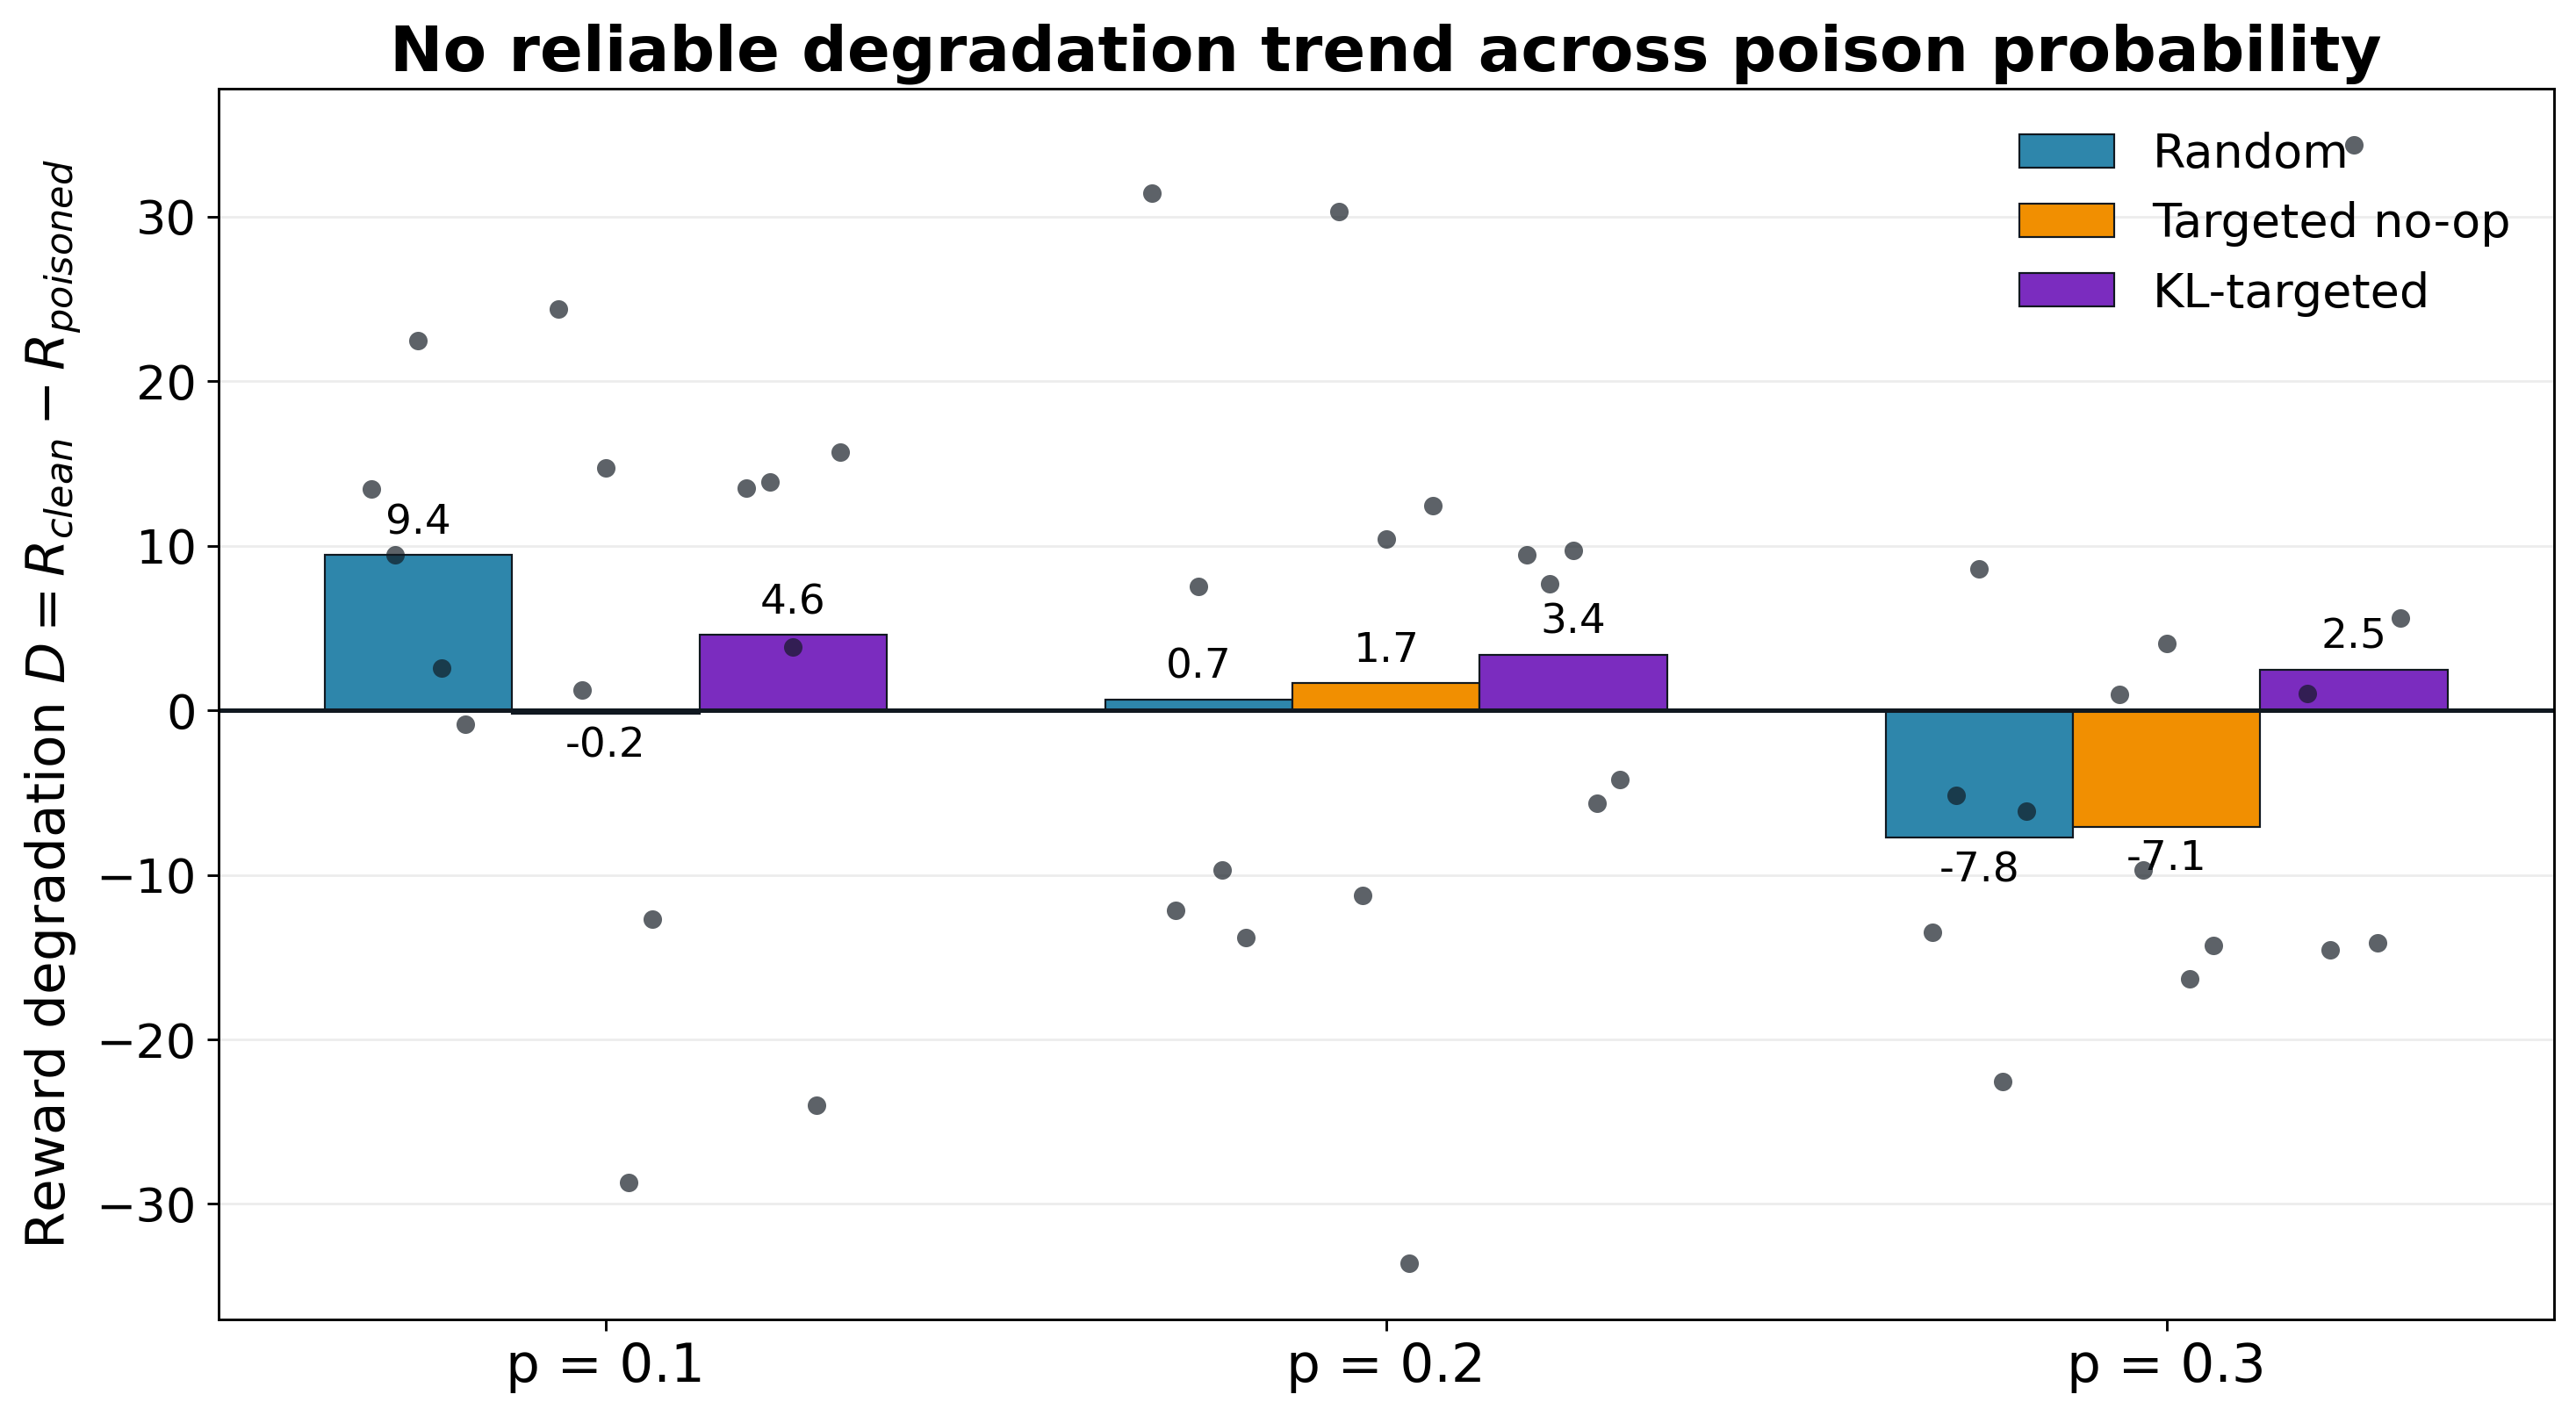
\includegraphics[width=0.92\linewidth]{figures/degradation_by_probability.png}
        \end{center}
        \tightcaption{Positive $D$ means the poisoned policy evaluated worse than the matched clean
        policy; negative $D$ means it evaluated better. Random and no-op are not reliably harmful
        and become negative on average at $p=0.3$.}

        \vspace{0.1em}
        \begin{center}
        \scriptsize
        \begin{tabular}{lrrrrr}
            \toprule
            $p$ & Random & Targeted no-op & KL-targeted & Any $D>0$ & All $D>0$ \\
            \midrule
            0.1 & 9.43 & -0.21 & 4.58 & 5/5 & 3/5 \\
            0.2 & 0.65 & 1.66 & 3.39 & 4/5 & 2/5 \\
            0.3 & -7.75 & -7.06 & 2.47 & 3/5 & 1/5 \\
            \bottomrule
        \end{tabular}
        \end{center}
        {\scriptsize Any $D>0$ = at least one attack degrades that matched seed. All $D>0$ = all three
        attacks degrade that matched seed.}

        \innerblock{What the plot supports}{
            \small
            \begin{itemize}
                \item Some settings degrade: several attack/$p$ averages have $D>0$.
                \item Degradation is not reliable: random and no-op become beneficial on average at $p=0.3$.
                \item Increasing $p$ does not increase degradation.
                \item KL-targeted has positive mean $D$ at all tested $p$, but not stable per-seed outcomes.
            \end{itemize}
        }

        \innerblock{Answer and caution}{
            \small
            Answer: sometimes, but not reliably. Positive examples exist, but many matched settings show
            no degradation or improvement. The data support mixed outcomes, not stable attack success.
        }
        \vspace{0.85em}
    }

    \block{6. Seed Sensitivity}{
        \begin{center}
            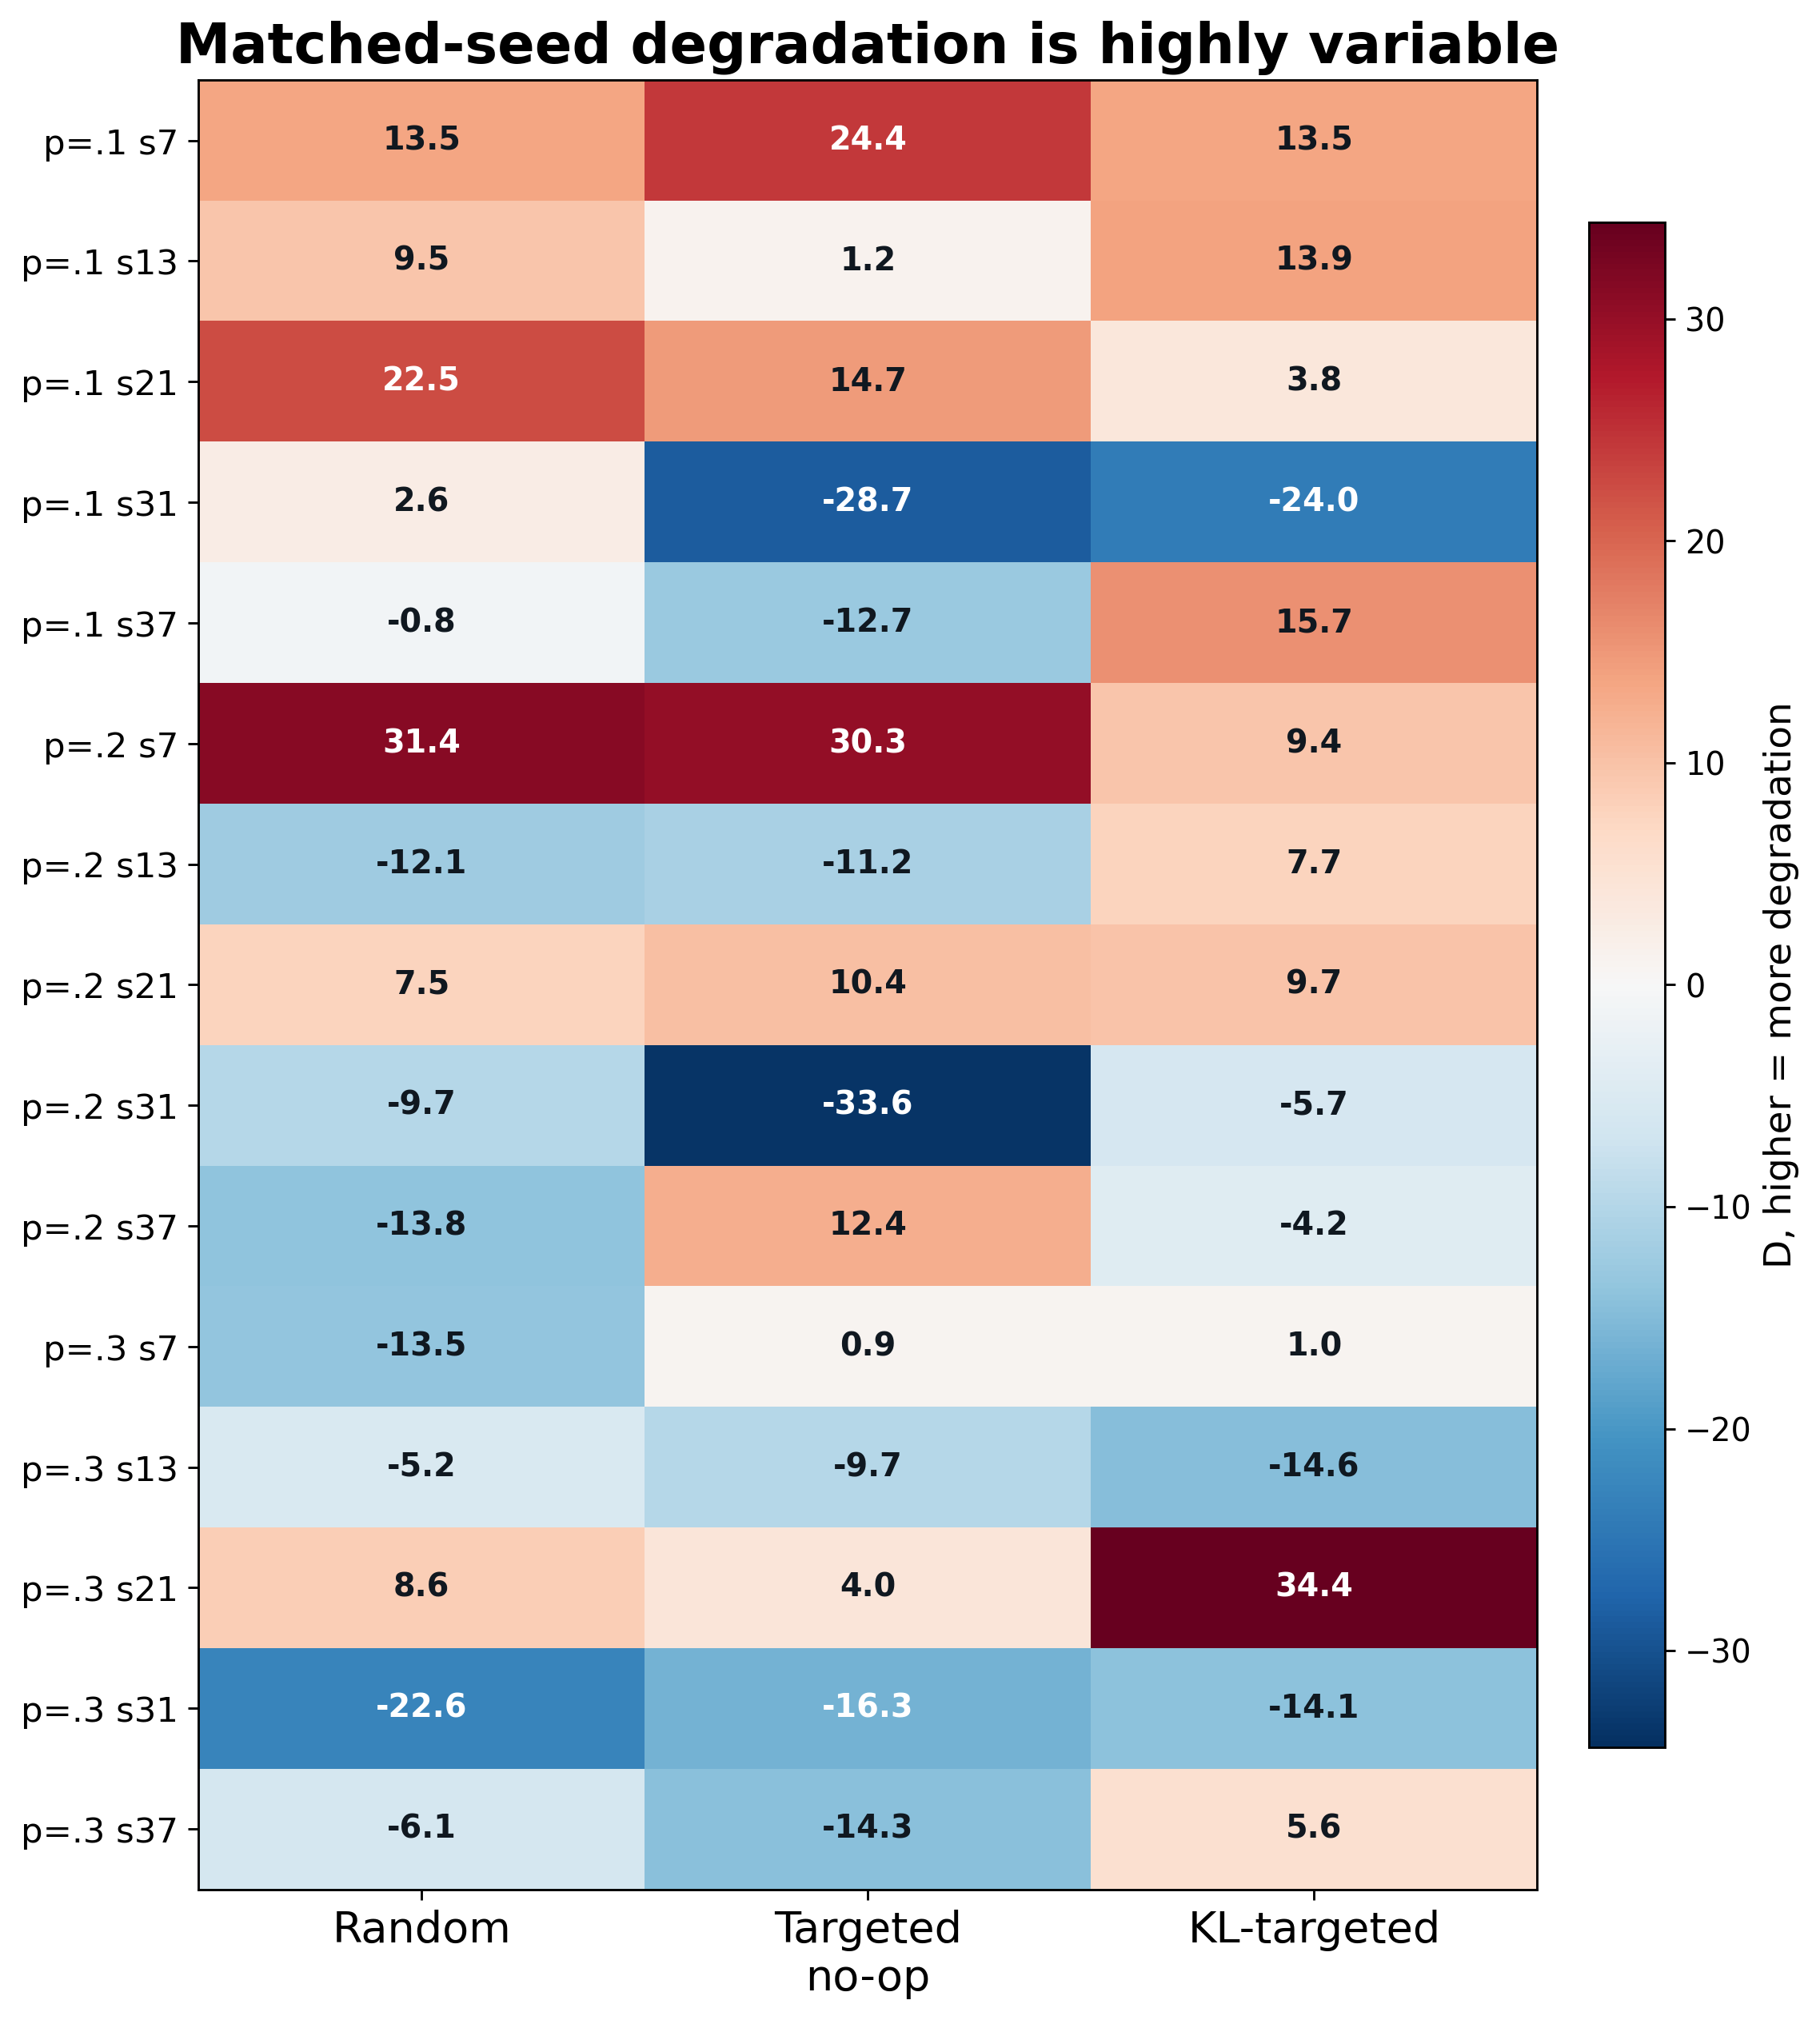
\includegraphics[width=0.45\linewidth]{figures/seed_heatmap.png}
        \end{center}
        \tightcaption{Each cell is matched-seed reward degradation. Red cells indicate degradation;
        blue cells indicate improvement over clean. The mixture shows highly seed-dependent outcomes.}

        \innerblock{Seed-level lesson}{
            \small
            Seed-level variation is the central observation: a single clean/poisoned comparison could
            overstate or understate the attack. Several negative cells mean stable degradation is not shown.
        }
    }

    \column{0.31}

    \block{7. Mechanism: Coverage and Collision Effects Are Noisy}{
        \begin{center}
            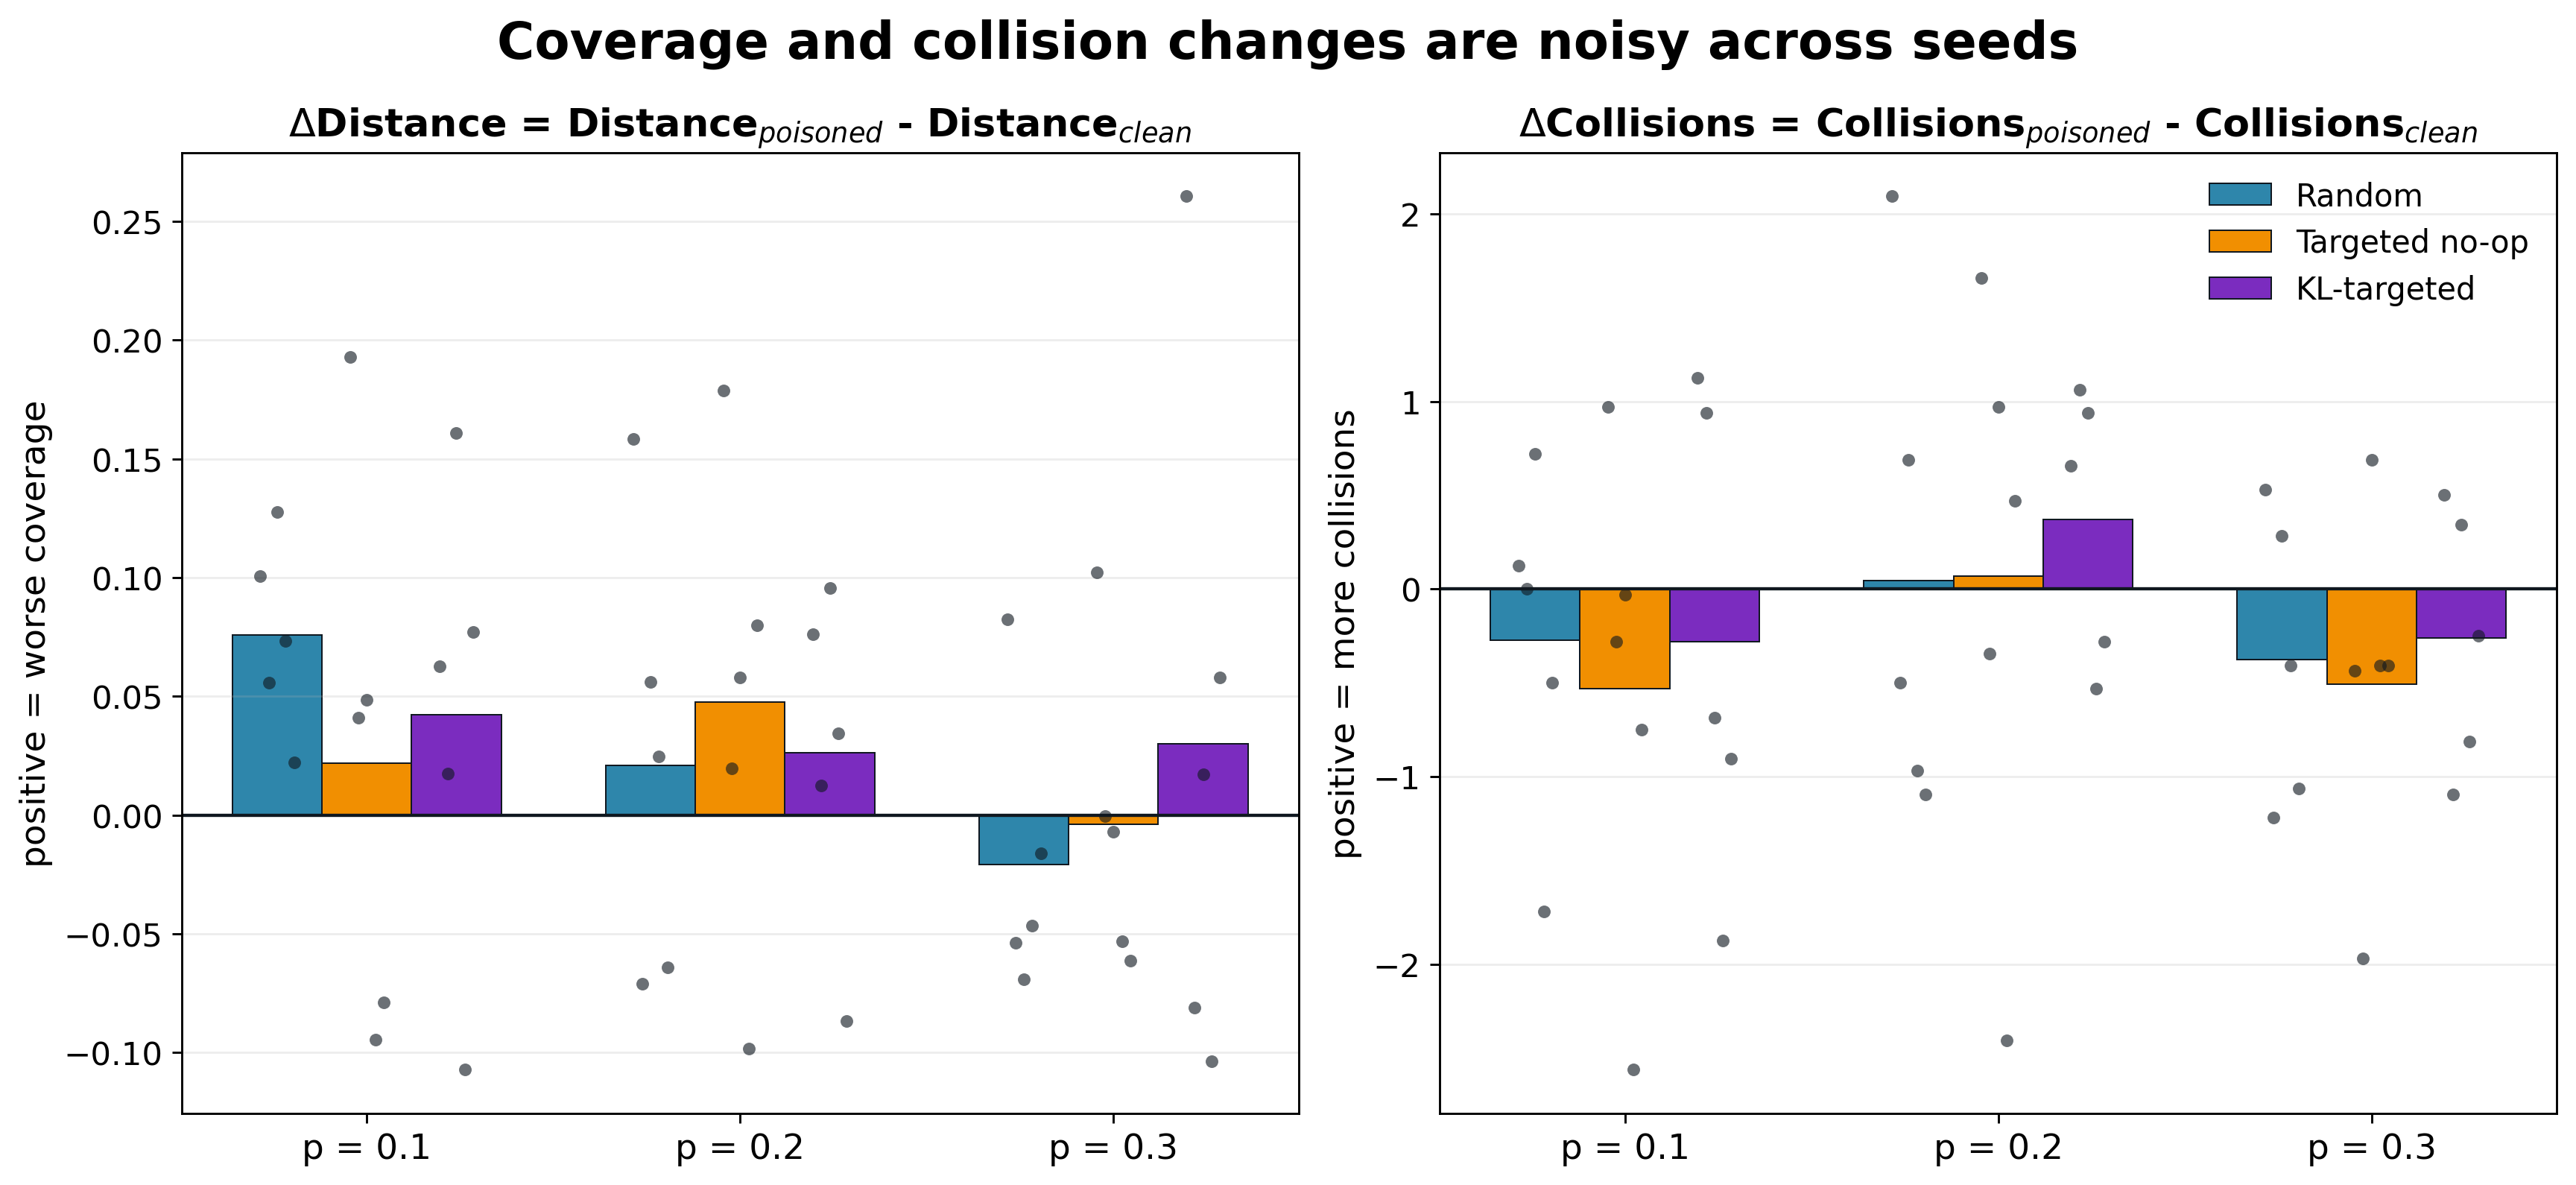
\includegraphics[width=1.00\linewidth]{figures/coverage_mechanism.png}
        \end{center}
        \tightcaption{Coverage and collision changes overlap across attacks and $p$ values. These plots
        do not reveal a simple mechanism that consistently explains reward degradation.}

        \begin{itemize}
            \item Reward includes both landmark coverage and collision penalties.
            \item Some poisoned policies improve one component while worsening another.
            \item Overlap is consistent with seed- and trajectory-dependent outcomes, but does not prove a mechanism.
        \end{itemize}

        \innerblock{Future defense ideas}{
            If future work finds stronger behavior-poisoning attacks, likely defenses would monitor rollout
            behavior rather than only rewards or gradients.
            \begin{itemize}
                \item Action-distribution anomaly detection.
                \item Per-agent entropy or intervention monitoring.
                \item Robust rollout filtering and adversarial teammate training.
            \end{itemize}
        }
        \vspace{0.45em}
    }

    \block{8. Hypothesis Check}{
        \begin{center}
        \footnotesize
        \begin{tabular}{p{0.34\linewidth}p{0.22\linewidth}p{0.34\linewidth}}
            \toprule
            Hypothesis & Outcome & Evidence \\
            \midrule
            H1 Clean MAPPO learns coordination & Baseline established & clean runs provide matched baselines \\
            H2 Poisoning reliably degrades clean evaluation & Not supported & many settings have $D \le 0$; random/no-op are negative at $p=0.3$ \\
            H3 No-op beats random & Not supported & no-op does not reliably produce higher $D$ \\ 
            H4 KL-constrained poisoning reliably degrades & Weak/mixed support & positive mean $D$ at all tested $p$, but variable by seed \\
            H5 More poison means more degradation & Not supported & average degradation decreases or reverses for random/no-op \\
            \bottomrule
        \end{tabular}
        \end{center}

        \innerblock{Bottom line}{
            Supported: non-monotonicity and seed sensitivity. Partially supported: some settings degrade.
            Not supported: reliable degradation, targeted dominance, or monotonic harm.
        }
        \vspace{0.85em}
    }

    \block{9. Takeaways, Limitations, and Next Steps}{
        \textbf{Takeaways}
        \begin{itemize}
            \item Action-level poisoning is a plausible training-time threat model, but this sweep did not show reliable degradation.
            \item Some matched-seed settings degrade clean-evaluation reward; many show no degradation or improvement.
            \item The most robust finding is non-monotonic, seed-sensitive behavior rather than stable attack success.
        \end{itemize}

        \textbf{Limitations:} one environment; one compromised agent; three $p$ values; one no-op target;
        five seeds; no confidence intervals. Conclusions are exploratory.

        \textbf{Next steps:} add seeds and confidence intervals; search target actions; compare against
        benign noise; test whether KL averages persist.

        \innerblock{Main lesson}{
            The attack model is plausible, but observed degradation is intermittent rather than reliable.
        }
    }
\end{columns}

\end{document}
